\section{\name Overview} \label{sec:overview}
\yueqiang{
requirements:
1) minimum modifications (SLoC);
2) keeping security (we need a short subsection to discuss the security)
3) minimum effects on page table allocation/deallocation in terms of memeory and CPU usage
}
\yueqiang{
algorithm: life cycle of pt cache (allocation, free)
pt cache(mechanism) enable and disable
}
%overview
Before we illustrate the design rationale of \name, we first describe the desired requirements that \name meets as follows:

R1) Retaining security. \name aims at reducing IOTLB flush while guaranteeing existing security strength.
R2) Achieving as good as possible performance. While benefitting IOTLB performance, \name is supposed to achieve positive results in the aspects of CPU and memory usage.
R3) Slightest possible modifications to Xen and Linux kernel for the sake of compatibility.

\subsection{Design Rationale}
In the \name, Xen enforces access control at a fine granularity to ensure security without flushing IOTLB. Besides, guest OS builds up cache pools to manage pages to support the fine-grained access control while facilitate the speed of every level of page table allocation/deallocation, saving CPU time while causing small impacts on memory usage.

\subsubsection{Fine-Grained Access Control}
%firstly, talk about how to reduce the IOTLB flush.
As revealed in previous sections, access control to writable pages is at a coarse granularity. Xen allows write-access both for guest OS and assigned I/O devices. Instead, \name caches a certain number of writable pages, prohibits DMA access for the cached writable pages while OS still has its write-permission. If they are updated to be page tables, Xen only limits OS to read-only permission (software protection) without modifying I/O page tables as well as IOTLB. Specifically, Xen maintains a new flag called \textbf{cache} with a machine page, indicating that the corresponding page is cached by guest OS and free from DMA-access. Whatever page type a machine page is, if it owns the flag, Xen neither maps nor unmaps it from I/O page tables, thus avoiding an IOTLB-flush. Note that \name only considers page type updates between WR-inter-PT.

For instance, if guest OS creates a new page-table, Xen firstly reuses the validation process to enforce software protection, and then checks if the page has the \textbf{cache} flag. If so, the only thing that Xen needs to do is to update the page to be a page-table. If not, Xen sets the page with the new flag, clears \emph{read} and \emph{write} permission fields in I/O page tables and flushes IOTLB. As for the guest page table destruction, Xen also reuses existing security checks to remove software protection, after which the corresponding page is set with the \textbf{cache} flag and updated to be writable while DMA prevention is still in effect. Figure \ref{fig:safe-flag} describes the process.

In this way, every time page type updates between WR-inter-PT occur, every related page will own the safe flag, 
 Xen only needs to revoke write-permission from the OS without unmapping the page from I/O page tables, theyexpensive IOTLB-flush. 

Also, \name proposes a novel cache algorithm in the guest OS to manage safe writable pages in order to prevent unacceptable exceptions caused by devices and facilitate the speed of creating/destructing page tables.
Ensuring security is demonstrated below.

\begin{figure}[ht]
\centering
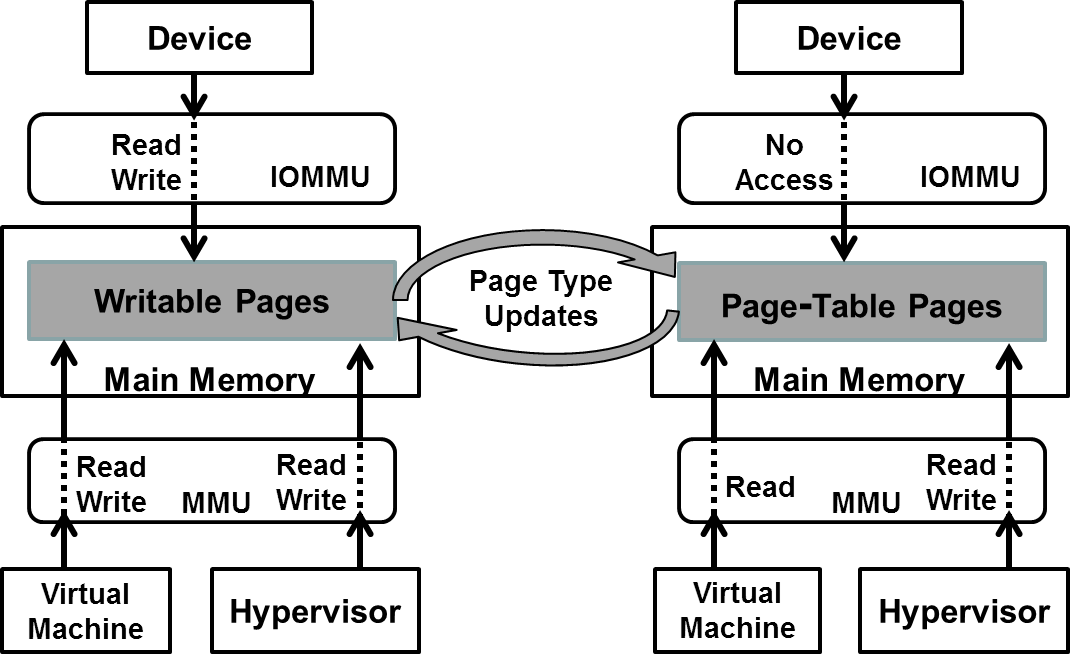
\includegraphics[width=0.5\textwidth]{image/background/wr2pt.png} \\
\caption{A Lifecycle of \textbf{cache} Flag}
\label{fig:safe-flag}
\end{figure}

\subsection{Cache Algorithm}
%secondly, design the cache pool to support it



enforce security polices in two aspects, i.e., guest OS and assigned I/O devices.Because of that, we associates the ready flag with

writable pages are writable for both guest OS and assigned I/O devices while

, , and  We defines that a writable page with a flag called \textbf{ready} that can be write-accessed by OS while inaccessible to devices. Because of that, when OS writes its writable pages with the ready flag (ready writable pages) as new page tables and submits the request of updating page tables, Xen reuses the existing validation process, however will not have to unmap them from I/O page tables instead the \textbf{ready} flag is marked with the page-table pages (ready page-table pages), thus reducing IOTLB-flushes. Besides, since the definition of page type is transparent to the OS, it needs to build a cache pool especially for the ready writable pages rather than free them into the buddy system which reserves only writable pages. Also, this cache mechanism benefits time efficiency when.

while provides every level of page-table cache pool for guest OS
